\documentclass[a4paper, fleqn]{article}
\usepackage[utf8]{inputenc}
\usepackage{amsmath}
\usepackage{amssymb}
\usepackage{caption}
\usepackage{mathtools}
\usepackage{amsfonts}
\usepackage{lastpage}
\usepackage{tikz}
\usepackage{float}
\usepackage{textcomp}
\usetikzlibrary{patterns}
\usepackage{pdfpages}
\usepackage{gauss}
\usepackage{fancyvrb}
\usepackage[table]{colortbl}
\usepackage{fancyhdr}
\usepackage{graphicx}
\usepackage{pdfpages}
\usepackage[margin=2.5 cm]{geometry}

\setlength\parindent{0pt}
\setlength\mathindent{75pt}

\definecolor{listinggray}{gray}{0.9}
\usepackage{listings}
\lstset{
	language=,
	literate=
		{æ}{{\ae}}1
		{ø}{{\o}}1
		{å}{{\aa}}1
		{Æ}{{\AE}}1
		{Ø}{{\O}}1
		{Å}{{\AA}}1,
	backgroundcolor=\color{listinggray},
	tabsize=3,
	rulecolor=,
	basicstyle=\scriptsize,
	upquote=true,
	aboveskip={0.2\baselineskip},
	columns=fixed,
	showstringspaces=false,
	extendedchars=true,
	breaklines=true,
	prebreak =\raisebox{0ex}[0ex][0ex]{\ensuremath{\hookleftarrow}},
	frame=single,
	showtabs=false,
	showspaces=false,
	showlines=true,
	showstringspaces=false,
	identifierstyle=\ttfamily,
	keywordstyle=\color[rgb]{0,0,1},
	commentstyle=\color[rgb]{0.133,0.545,0.133},
	stringstyle=\color[rgb]{0.627,0.126,0.941},
  moredelim=**[is][\color{blue}]{@}{@},
}

\lstdefinestyle{base}{
  emptylines=1,
  breaklines=true,
  basicstyle=\ttfamily\color{black},
}

\pagestyle{fancy}
\def\checkmark{\tikz\fill[scale=0.4](0,.35) -- (.25,0) -- (1,.7) -- (.25,.15) -- cycle;}
\newcommand*\circled[1]{\tikz[baseline=(char.base)]{
            \node[shape=circle,draw,inner sep=2pt] (char) {#1};}}
\newcommand*\squared[1]{%
  \tikz[baseline=(R.base)]\node[draw,rectangle,inner sep=0.5pt](R) {#1};\!}
\newcommand{\comment}[1]{%
  \text{\phantom{(#1)}} \tag{#1}}
\def\el{[\![}
\def\er{]\!]}
\def\dpip{|\!|}
\def\MeanN{\frac{1}{N}\sum^N_{n=1}}
\cfoot{Page \thepage\ of \pageref{LastPage}}
\DeclareGraphicsExtensions{.pdf,.png,.jpg}
\author{Nikolaj Dybdahl Rathcke (Student ID: 74763954)}
\title{Cryptography and Coding Theory \\ Assignment 1}
\lhead{Cryptography and Coding Theory}
\rhead{Assignment 1}

\begin{document}

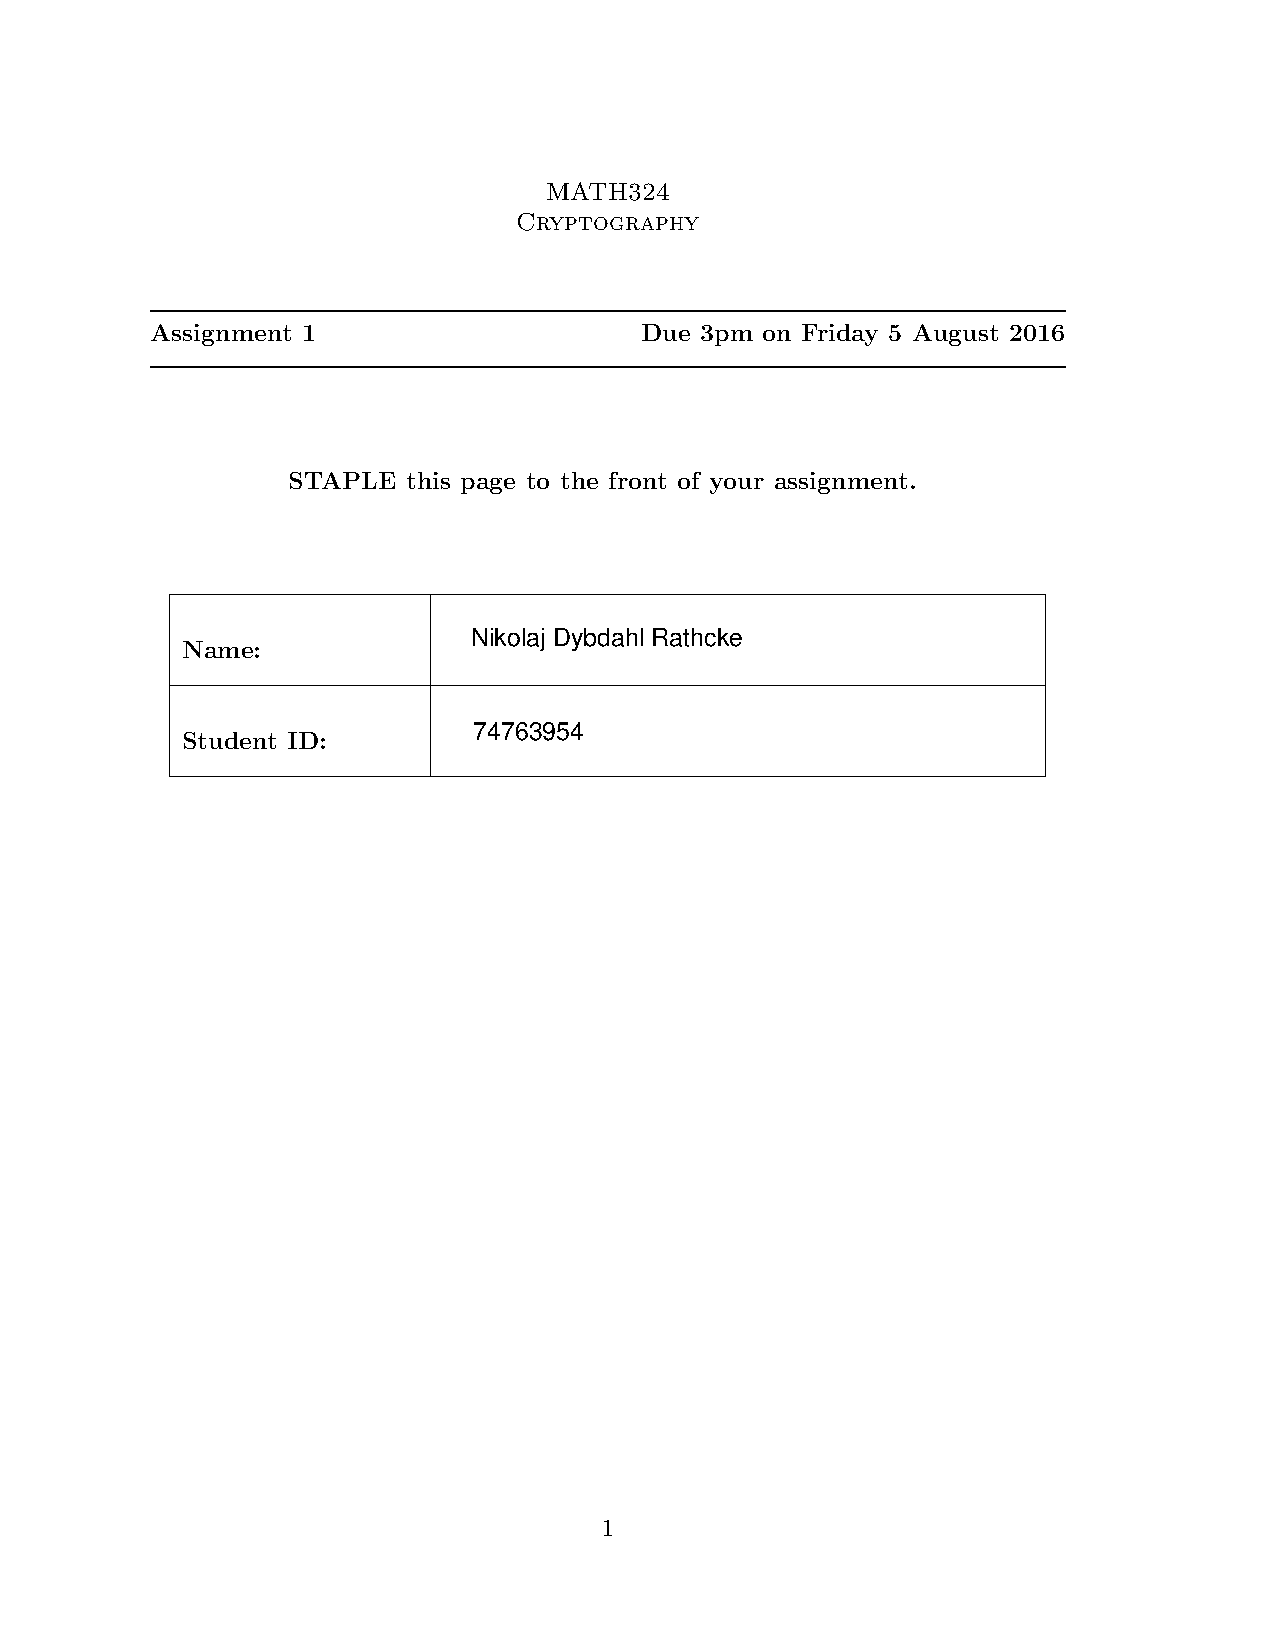
\includepdf[pages=1]{title.pdf}

\section{Question 1}
\subsection{(i)}
Both Diffie-Hellman and ElGamal uses modular exponentation and they both rely on the diffuculty of breaking the discrete logarithm problem. They are similar in the sense that both of them are public-key protocols, though Diffie-Hellman is an example of public key-exchange while ElGamal is a public-key encryption scheme. \\
The difference is that Diffie-Hellman is a protocol where two people compute a common secret, whereas ElGamal uses the public keys to encrypt a message as a one-time thing. This means that we do not need both people to be present in the exchange for ElGamal, but we do for Diffie-Hellman.

\subsection{(ii)}
The encryption of a message $m$ works by taking the public key $(G, g, A)$ and choosing a random $b\in \{1,\ldots, |G|-1\}$ and then calculating $B=g^b$ as well as $c=A^bm$ (the encryption function) where $A=g^a$). The decryption works by computing $m=(B^a)^{-1}c$ (the decryption function). \\
To prove they are inverse function, we need to show that:
\begin{align*}
  f(g(x))=x \mbox{ and } g(f(x))=x
\end{align*}
This means we have $f(x)=A^bx$ and $g(x)=(B^a)^{-1}x$. Calculating $f(g(x))$ gives:
\begin{align*}
  A^b((B^a)^{-1}x) &= (g^a)^b(((g^b)^a)^{-1}x) \\
                   &= g^{ab}g^{-ba}x \\
                   &= x
\end{align*}
And calculating $g(f(x))$ gives us:
\begin{align*}
  (B^a)^{-1}(A^bx) &= ((g^b)^a)^{-1}((g^a)^bx) \\
                   &= g^{-ba}g^{ab}x \\
                   &= x
\end{align*}
which proves that the two functions are inverse operations.

\subsection{(iii)}\label{ref1}
It is not required that $g$ is a generator for the cryptosystem to be safe. However, if the order of $g$ is composed of small prime factors, the Discrete Logarithm Problem becomes easy to solve (using algorithms like Pohlig–Hellman). Thus, it is important that the order of $g$ has a large prime factor.

\subsection{(iv)}
If the Discrete Logarithm Problem was not hard, an attacker would be able to compute the secret $a$. If the attacker could snatch the cyphertext pair $(B, c)$, it could then easily be decoded. But since the problem is believed to be hard, even if the encrypted message went through a middle-man, he is not able to decrypt it.

\section{Question 2}

\subsection{(i)}
The prime $p$ is the number $503$. There are several ways to check if a number is prime. One well-known way is to see if a number $n$ is prime is by checking if any of the primes less than the square root of $n$ divides $n$. We could also use a primality test such as miller-rabin, which works well in this case as it is correct if it outputs a $n$ is composite, but could be wrong if it outputs that $n$ is prime (I was so lucky to have this lying around). There are also deterministic versions of primality tests. \\
Choosing a cyclic group $(Z/pZ)^*$ for a prime $p$ is important as it means $\phi(p)=p-1$, i.e. that all members in the group are coprime with $p$. Thus, when we pick the generator $g$, we ensure that the final secret number can have any value from $1$ to $p-1$.

\subsection{(ii)}
An algorithm \cite[Algorithm 2.5.16]{wstein} I found which finds the smallest element $g$ that generates $(Z/pZ)^*$ gives the following approach:
\begin{enumerate}
  \item  $[p = 2?]$ If $p=2$ output $1$ and terminate. Otherwise set $a=2$.
  \item  $[\mbox{Prime Divisors}]$ Compute the prime divisors $p_1,\ldots, p_r$ of $p-1$.
  \item  $[\mbox{Generator?}]$ If for every $p_i$, we have $a^{(p-1)/p_i} \not\equiv 1$ (mod $p$), then $a$ is a generator of $(Z/pZ)^*$, so output $a$ and terminate.
  \item  $[\mbox{Try next}]$ Set $a=a+1$ and go to Step 3.
\end{enumerate}
The prime factors, $p_i$ of $p-1=502$ is $2$ and $251$. This means there are $\varphi(502)=502(1-\frac{1}{2})(1-\frac{1}{251}=250$ primitive roots, so we should hopefully not need too many iterations of the algorithm. Table \ref{tab1} shows the calculations made in step $3$ of the algorithm:
\begin{table}[H]
  \centering
  \begin{tabular}{|c|c|c|}
  \hline
  $a$ & $a^{502/2}$ mod $503$ & $a^{502/251}$ mod $503$ \\
  \hline
  $2$ & $1$ & \\
  \hline
  $3$ & $1$ & \\
  \hline
  $4$ & $1$ & \\
  \hline
  $5$ & $502$ & $25$ \\
  \hline
  \end{tabular}
  \caption{Table showing the calculations made in step $3$ of the above algorithm.}
  \label{tab1}
\end{table}
And the algorithm terminates. The number $5$ is a generator for the cyclic group.

\subsection{(iii)}
Let us randomly choose $a=41$, meaning we get $5^{41} \equiv 304$ mod $503$. So we have $A=304$ and our public key is $(503, 5, 304)$.

\section{Question 3}

\subsection{(i)}
Yes, she can recover $m_2$. If we use the same element $b$, that means the two cyphertext pairs are $(B_1, c_1) = (g^b, A^b\cdot m_1)$ and $(B_2, c_2)=(g^b, A^b\cdot m_2)$. As Eve knows $m_1$ and $c_1$, that means she also knows $m_1^{-1}$ (in $(Z/pZ)^*$. Using this, she compute $A^b=c_1\cdot m_1^{-1}$. Knowing this secret, she can simply calculate $(A^b)^{-1}$ and find $m_2=c_2(A^b)^{-1}$.

\subsection{(ii)}
This is easy to do as the ElGamal encryption is \textit{malleable}, which means it is possible to transform one cyphertext into another valid cyphertext.meaning if we intercept the ciphertext $(B, c)$, we simply compute $(B, 2c)$ as it is a valid encryption of $2m$. It is easy to see this as $2c=(2m)A^b$. \\
It is possible to transform ElGamal into a hashed version (one well-known is the Cramer–Shoup cryptosystem) to attempt to defend yourself against these kind of attacks.

\section{Question 4}
We will focus on two algorithms for computing the discrete logarithm, that is, finding $x$ in $g^x\equiv a$ (mod $p$). These are the Pohlig-Hellman algorithm and the Index calculus algorithm, which will be explained conceptually.

\subsection{Pohlig-Hellman}
As mentioned in section \ref{ref1}, an algorithm for computing discrete logarithm when the order of the multiplicative group is a \textit{smooth integer} (that its prime factorization is composed of small primes) is the Pohlig-Hellman algorithm \cite{pohlig}. \\
The algorithm utilizes the Chinese remainder theorem, which states that if we have integers $a,b,n$ and $m$, so that:
\begin{align*}
  x&\equiv a \mbox{ (mod $n$)} \\
  x&\equiv b \mbox{ (mod $m$)}
\end{align*}
Then we can uniquely determine $x$. For Pohlig-Hellman, we compute the prime factorization (which should be easy as they are small primes). Say the prime factors are $q_1^{a_1}$ and $q_2^{a_2}$, we can then determine
\begin{align*}
  x_1 &= x \mbox{ mod } q_1^a \\
  x_2 &= x \mbox{ mod } q_2^b
\end{align*}
by calculating $a^((p-1) / q)$, which we know. When we obtain all necessary $x_i$, we can use the Chinese remainder theorem to work out $x$. \\
\\
The algorithm runs in $\mathcal{O}(\sqrt{n})$ time for group order $n$. If the order is smooth, we can give an alternative worst-case running time. Say $\prod_i q_i^{a_i}$ is the prime factorization, then it runs in $\mathcal{O}\left( \sum_i a_i(\lg n + \sqrt{p_i})\right)$ \cite{menezes}.

\subsection{Index Calculus}
The index calculus algorithm is a probabilistic algorithm \cite[pp. 109-110]{menezes} for computing the discrete logarithm. The idea here is that we give the algorithm a \textit{factor base} as input. This factor base, $S$ contains all primes, $p_1, p_2,\ldots p_n$, which are less than a given $k$ (and usually, it will also contain $-1$). The idea is then to pre-compute a database by finding the logarithms of the elements in $S$. We then try to write $g^k$ as a product of elements in $S$:
\begin{align*}
  g^k \equiv \prod_i^n p_i^{k_i}
\end{align*}
for random $k\in \{1,\ldots, p-1\}$. If we are able to do so, we can take the logarithm of both sides to get a linear relation (with $1$ unknown). \\
When we have more than $n+1$ relations, we can construct a linear system and solve it as we have $n$ unknowns. \\
Next, we search for a power $s$ of the generator, so that $ag^s$ can be factored using the factor base. That is, we try to
\begin{align}\label{eq1}
  ag^s\equiv \prod_i^n p_i^{k_i}
\end{align}
If this is successfull, we can finally compute the discrete logarithm by some algebraic manipulation of Equation \ref{eq1}. \\
\\
The running time of the algorithm depends a lot of things. We need to pick $n$, the size of the factor base, carefully. With an optimal choice of this parameter, we can expect it to run in (L-notation) $L_q[1/2, c]$ for some constant $c$, when $q=p$ or $q=2^m$ \cite[p. 112]{menezes}.

\begin{thebibliography}{9}

  \bibitem{wstein}
  Stein, William. Elementary Number Theory: Primes, Congruences, and Secrets: A Computational Approach. Springer Science \& Business Media, 2008.

  \bibitem{pohlig}
  Pohlig, Stephen, and Martin Hellman. "An improved algorithm for computing logarithms over GF(p) and its cryptographic significance (Corresp.)." IEEE Transactions on information Theory 24.1 (1978): 106-110.

  \bibitem{menezes}
  Menezes, Alfred J., Paul C. Van Oorschot, and Scott A. Vanstone. Handbook of applied cryptography. CRC press, 1996.

\end{thebibliography}

\end{document}
